%%%%%%%%%%%%%%%%%%%%%%%%%%%%%%%%%%%%%%%%%
% kaobook
% LaTeX Template
% Version 1.3 (December 9, 2021)
%
% This template originates from:
% https://www.LaTeXTemplates.com
%
% For the latest template development version and to make contributions:
% https://github.com/fmarotta/kaobook
%
% Authors:
% Federico Marotta (federicomarotta@mail.com)
% Based on the doctoral thesis of Ken Arroyo Ohori (https://3d.bk.tudelft.nl/ken/en)
% and on the Tufte-LaTeX class.
% Modified for LaTeX Templates by Vel (vel@latextemplates.com)
%
% License:
% CC0 1.0 Universal (see included MANIFEST.md file)
%
%%%%%%%%%%%%%%%%%%%%%%%%%%%%%%%%%%%%%%%%%

%----------------------------------------------------------------------------------------
%	PACKAGES AND OTHER DOCUMENT CONFIGURATIONS
%----------------------------------------------------------------------------------------

\documentclass[
	a4paper, % Page size
	fontsize=10pt, % Base font size
	twoside=false, % Use different layouts for even and odd pages (in particular, if twoside=true, the margin column will be always on the outside)
	%open=any, % If twoside=true, uncomment this to force new chapters to start on any page, not only on right (odd) pages
	%chapterentrydots=true, % Uncomment to output dots from the chapter name to the page number in the table of contents
	numbers=noenddot, % Comment to output dots after chapter numbers; the most common values for this option are: enddot, noenddot and auto (see the KOMAScript documentation for an in-depth explanation)
]{kaobook}
\usepackage{array}
\usepackage{tikz}
\newcolumntype{P}[1]{>{\raggedright\arraybackslash}p{#1}}

% Choose the language
\ifxetexorluatex
	\usepackage{polyglossia}
	\setmainlanguage{english}
\else
	\usepackage[english]{babel} % Load characters and hyphenation
\fi
\usepackage[english=british]{csquotes}	% English quotes

% Load packages for testing
\usepackage{blindtext}
%\usepackage{showframe} % Uncomment to show boxes around the text area, margin, header and footer
%\usepackage{showlabels} % Uncomment to output the content of \label commands to the document where they are used

% Load the bibliography package
\usepackage{kaobiblio}
\addbibresource{main.bib} % Bibliography file

\usepackage{enumitem}
\usepackage{float}
% Load mathematical packages for theorems and related environments
\usepackage[framed=true]{kaotheorems}

% Load the package for hyperreferences
\usepackage{kaorefs}

\graphicspath{{examples/documentation/images/}{images/}} % Paths in which to look for images

\makeindex[columns=3, title=Alphabetical Index, intoc] % Make LaTeX produce the files required to compile the index

\makeglossaries % Make LaTeX produce the files required to compile the glossary
\newglossaryentry{computer}{
	name=computer,
	description={is a programmable machine that receives input, stores and manipulates data, and provides output in a useful format}
}

% Glossary entries (used in text with e.g. \acrfull{fpsLabel} or \acrshort{fpsLabel})
\newacronym[longplural={Frames per Second}]{fpsLabel}{FPS}{Frame per Second}
\newacronym[longplural={Tables of Contents}]{tocLabel}{TOC}{Table of Contents}

 % Include the glossary definitions

\makenomenclature % Make LaTeX produce the files required to compile the nomenclature

% Reset sidenote counter at chapters
%\counterwithin*{sidenote}{chapter}

%----------------------------------------------------------------------------------------
\usepackage{svg}
\pagelayout{wide} % No margins
\pagelayout{margin} % Restore margins
\setlength{\marginparwidth}{0pt} % Imposta la larghezza della colonna marginale a 0
\setlength{\marginparsep}{0pt}   % Rimuovi lo spazio tra il testo principale e la colonna marginale
\usepackage[utf8]{inputenc}
\usepackage[T1]{fontenc}
\usepackage{ebgaramond}
\usepackage{fontspec}                                                                                                                       
\addtokomafont{title}{\sffamily}
\addtokomafont{chapter}{\sffamily}
\addtokomafont{section}{\sffamily}
\addtokomafont{subsection}{\sffamily}
\addtokomafont{subsubsection}{\sffamily}
\begin{document}
\setmainfont{EB Garamond}

%----------------------------------------------------------------------------------------
%	BOOK INFORMATION
%----------------------------------------------------------------------------------------

\titlehead{Requirement Analysis and Specification
	Document}

\title[Requirement Analysis and Specification
Document]{Requirement Analysis and Specification
	Document}
\subtitle{Students\&Companies project Andrea Bellani Alessandro Capellino}

\author[Andrea Bellani, Alessandro Capellino]{Andrea Bellani, Alessandro Capellino}

\date{\today}


\includegraphics[scale=0.3]{Politecnico.png}


\publishers{Politecnico di Milano}

%----------------------------------------------------------------------------------------

\frontmatter % Denotes the start of the pre-document content, uses roman numerals

%----------------------------------------------------------------------------------------
%	OPENING PAGE
%----------------------------------------------------------------------------------------

%\makeatletter
%\extratitle{
%	% In the title page, the title is vspaced by 9.5\baselineskip
%	\vspace*{9\baselineskip}
%	\vspace*{\parskip}
%	\begin{center}
%		% In the title page, \huge is set after the komafont for title
%		\usekomafont{title}\huge\@title
%	\end{center}
%}
%\makeatother

%----------------------------------------------------------------------------------------
%	COPYRIGHT PAGE
%----------------------------------------------------------------------------------------

\makeatletter
\uppertitleback{\@titlehead} % Header

\lowertitleback{
	\textbf{Copyright}\\
	\cczero\ 2024, Andrea Bellani Alessandro Capellino – All rights reserved \\
	
	The entire project is available at
	\\\url{https://github.com/ImAndreaBellani/BellaniCapellino}
	
	\textbf{Publisher} \\
	First printed in \today\ by \@publishers
}
\makeatother

%----------------------------------------------------------------------------------------
%	DEDICATION
%----------------------------------------------------------------------------------------

%----------------------------------------------------------------------------------------
%	OUTPUT TITLE PAGE AND PREVIOUS
%----------------------------------------------------------------------------------------

% Note that \maketitle outputs the pages before here

\maketitle

%----------------------------------------------------------------------------------------
%	PREFACE
%----------------------------------------------------------------------------------------

%----------------------------------------------------------------------------------------
%	TABLE OF CONTENTS & LIST OF FIGURES/TABLES
%----------------------------------------------------------------------------------------

\begingroup % Local scope for the following commands

% Define the style for the TOC, LOF, and LOT
%\setstretch{1} % Uncomment to modify line spacing in the ToC
%\hypersetup{linkcolor=blue} % Uncomment to set the colour of links in the ToC
\setlength{\textheight}{230\hscale} % Manually adjust the height of the ToC pages

% Turn on compatibility mode for the etoc package
\etocstandarddisplaystyle % "toc display" as if etoc was not loaded
\etocstandardlines % "toc lines" as if etoc was not loaded

\tableofcontents % Output the table of contents

\listoffigures % Output the list of figures

% Comment both of the following lines to have the LOF and the LOT on different pages
\let\cleardoublepage\bigskip
\let\clearpage\bigskip

\listoftables % Output the list of tables

\endgroup

%----------------------------------------------------------------------------------------
%	MAIN BODY
%----------------------------------------------------------------------------------------

\mainmatter % Denotes the start of the main document content, resets page numbering and uses arabic numbers
\setchapterstyle{kao} % Choose the default chapter heading style

\pagelayout{wide} % No margins
\chapter{Introduction}
\labch{intro}
	\section{Purpose}
		During their university studies, in order to start entering the workforce, a student might decide to apply for an internship related to their field of study. Similarly, companies offering internships may be interested in finding students that are adequate for them. To facilitate the matching between students and companies, a new platform called \emph{Students and Companies} (S\&C) is to be developed. S\&C allows companies to look for suitable students by publish internship advice on the platform, while students can look for internships that interest them. Moreover, the platform implements recommendation mechanism to help student and companies to find each other. Once the contact is established, S\&C can provide support to the students selection process.
		\subsection{Goals}
			The main goals of the system are:
			
			\quad [G1]\quad students and companies establish contacts for doing internships;
			
			\quad [G2]\quad internships selections can be monitored and supported by the system;
			
			\quad [G3]\quad ongoing internships can be monitored from the system.
	\section{Scope}
		In this section, we are identifying the S\&C domain. In particular, there are two main users categories that interact with the system: \emph{Companies} and \emph{Students}. The companies publish announcements about the internships they want to offer where they specify \emph{projects} that will be carried out and the \emph{terms} of the offer. The system itself informs the companies about the availability of students who may be suitable for their internships (based on their profile).
		
		Students, on the other hand, may use the platform to look for internships and S\&D can also notify them if there are new internships that could meet their interests, but they can still independently search through all the available internships.
		
		Once a \emph{contact} is established and accepted by the two parties, the student selection process begins. At this point the company defines selection steps and schedules the interviews for each student. Once the selection is over, the system collects feedback and suggestions from both students and companies.
		
		Finally, both students and companies can monitor the progress of the internships by providing information on its development and any issues that may arise.
		\subsection{Phenomena}
			\subsubsection{World Phenomena}
			\subsubsection{Shared Phenomena}
				\paragraph{World-controlled Shared Phenomena}
				\paragraph{Machine-controlled Shared Phenomena}
	\section{Definitions, Acronyms and Abbreviations}
		\subsection{Definitions}
			\begin{itemize}
				\item \textbf{internship advice} : a call for application related to an internship that will be offered by a company;
				\item \textbf{recommendation} : the mechanism related to the fact that the system both informs students whether new internship advice that might interest them are published and notifies companies of the presence of students that might be suitable for their internships;
				\item \textbf{project} (of an internship advice) : the definition of the application domain, the set of tasks to be performed and the set of the most relevant adopted technologies (if any) for an internship;
				\item \textbf{terms} (of an internship advice) : the set of benefits offered by an internship (e.g. paid/not paid, training, lunch voucher... );
				\item \textbf{selection process} : each internship advice is followed by a sequence of selection steps.
			\end{itemize}
		\subsection{Acronyms}
			\begin{itemize}
				\item S\&C: Students\&Companies, the name of the platform;
				\item UML: Unified Modeling Language;
				\item CV: Curriculum Vitae.
			\end{itemize}
		\subsection{Abbreviations}
			\begin{itemize}
				\item Gn: Goal number n;
				\item Rn: Requirement number n;
				\item Dn: Domain assumption number n;
				\item WPn: World Phenomena number n;
				\item SPn: Shared Phenomena number n;
				\item UC: Use Case.
			\end{itemize}
	\section{Revision history}
	\section{Reference documents}
		The Documents used to deliver the RASD document are the following:
		\begin{itemize}
			\item the Specification of RASD and DD assignment of Software Engineering 2;
			\item the class slides on WeBeep, in particular slides on RE (requirement engineering), scenarios and Use Cases and UML diagrams;
		\end{itemize}
	\section{Document structure}
		\begin{enumerate}
			\item \textbf{Introduction}: this section provides a brief introduction to the purpose of the platform to be developed, S\&C in this case, focusing in particular on the most important goals which the system has to achieve and on the various phenomena identified;
			\item \textbf{Overall Description} : an high-level (conceptual) description of the system functionalities explained through scenarios, high-level class diagram, product functions and domain assumption;
			\item \textbf{Specified Requirements} : the detailed requirements analysis. In this section is detailed the entire requirement set (functional and non-functional), the most relevant use-cases (including sequence diagrams that formalize them) and the design constraints that must be stated also at the requirement level;
			\item \textbf{Formal Analysis} : formal modeling and simulation of a simplified model of the system, in order to formally prove the correctness of the (possibly) foremost requirements (using Alloy 6);
			\item \textbf{Effort Spent}: report of the time spent by any group member in any document section;
			\item \textbf{References}: list of software and documents used to develop the document.
		\end{enumerate}
\chapter{Overall description}
\labch{options}
	\section{Product perspective}
		\subsection{Scenarios}
			\textbf{Student signs up to S\&C}
			\begin{flushleft}
				Student Bob enters in the system for the first time. On the homepage, he first clicks the \emph{Registration button} and then the \emph{Student Registration button}. To register, Bob fills out a form providing its institutional e-mail (bob.johnson@mail.polimi.it) and password (which will be used for future logins), a brief description of his academic background and specifies whether he would like to take part to the recommendation analysis. Finally, Bob uploads his CV by clicking the \emph{Upload CV button}. Now Bob is registered and can search for internships that interest him.
			\end{flushleft}
			\textbf{Company signs up to S\&C}
			\begin{flushleft}
				The company FinestraMI enters the system for the first time. On the homepage, it first clicks the \emph{Registration button} and then the \emph{Company Registration button}. To register, the company fills out a form providing its name, a brief description of its area of expertise and its business area (the market where it operates) and finally its corporate e-mail (info@finestrami.it) and password (which will be used for future logins). FinestraMI also specifies, by selecting the appropriate option, whether it wants take part into the recommendation analysis. Now, FinestraMI is registered and can publish its internships advice.
			\end{flushleft}
			\textbf{Company publishes an internship offer}
			\begin{flushleft}
				The company FinestraMI enters in the system; on the homepage, it clicks the \emph{Login button}. Once logged in, FinestraMI accesses the \emph{Publish New Internship section}. A new internship advice is added by filling out a form where the following information is provided:
				\begin{itemize}
					\item "Window restore" (the intership title);
					\item "The aim of this internship is to give to student to opportunity to repair office windows and..." (a brief description);
					\item "third year bachelor students..." (experience required);
					\item "not suffering from dizziness" (desired skills);
					\item "1. coordination of glass disposal; 2. ..." (main activities the internship involves);
					\item "no paid, canteen tickets available" (terms of the internship);
					\item "22/11/2024" (advice deadline).
					\item max 42 applications (max number of applications)				
					\end{itemize}
				
				Now the internship advice is visible to students registered on the platform (and also to FinestraMI).
			\end{flushleft}
			\textbf{Student proactively searches for an internship}
			\begin{flushleft}
				Students Bob, Alice and Micheal access to the system by clicking "Login". Each one of them wants to find an internship to apply but each one of them has a different idea of what and where he/she would like to do/be:
				\begin{itemize}
					\item Bob is really interested on doing practice on an handwork but he neither knows a name of a company nor knows which kind of handwork apply for so, he goes to the \emph{View Internships section}, where he can see all the published internships, listed from the most recent to the least recent. The most recent one is "Window restore" by FinestraMI, then he selects it;
					\item Alice has not already decided the kind of internship she wants to apply for but knows many names of companies that operate near her home and so she prefers to go to the \emph{View Companies section}, where she can see all the registered companies and all the internships published by each company. Then she recognized FinestraMI and since she knows that it is expanding, she decides to select it. "Window restore" is the only available advice of FinestraMI but she select it anyways;
					\item Micheal is looking forward to do an internship related to windows restoration, so he uses the search bar to insert "windows restoration" and selects the option "only paid internships", but no internship are found. Then he removes the option and find the internship of FinestraMI. Since it is the only left, he selects it.
				\end{itemize} 
			\end{flushleft}
			\textbf{Student receive a notification about a new internship}
			\begin{flushleft}
				The company CancellaMI (previously registered to the platform) publishes a new internship related to railings maintenance then, Student Bob, who has chosen to be notified by the system when new internships that might be of interest are published, receives an email informing it that a new intership related to his studies is available, since it stated in his CV that after the internship at FinestraMI he became passionate of railings. Bob then logs into the platform and, by going to the \emph{Notification section}, can view the internships offer in more detail.
			\end{flushleft}
			\textbf{Company receives a notification about new possibly interested students}
			\begin{flushleft}
				Company FinestraMI, which has chosen to be notified by the system, receives an email informing it that new students are appealing for its intership "Window Restore" (based on their CVs). FinestraMI then logs into the platform, goes into the \emph{Internship section}, clicks on \emph{Windows restore internship} and by going to the \emph{Notification section} can view the students'profiles and their CVs in more detail.
			\end{flushleft}
			\textbf{Student applies for an internship}
			\begin{flushleft}
				Student Bob wants to apply for the internship "Windows restore". To do so, they log into the system, access the page for "Windows restore" internship and click the \emph{Apply button}. Automatically, the system will send a notification to FinestraMI (the company offering the internship) to inform it that Bob has applied
			\end{flushleft}
			\textbf{The company accepts the application of a student}
			\begin{flushleft}
				Company FinestraMI receives the email regarding student Bob's application for the internship "Window Restore". FinestraMI then logs into the platform, navigates to the \emph{Internships section}, select the \emph{Window Restore Internship}, goes to the \emph{Notification section} and clicks the \emph{Accept Application button} to approve Bob's application.
			\end{flushleft}
			\textbf{The company proposes to a student to apply for one of its internships}
			\begin{flushleft}
				The company FinestraMI consults its list of recommended students for Window Restore and send a proposal to Bob Jones (by clicking on the dedicated button). Soon after the system sends a notification of the proposal to Bob. 
			\end{flushleft}
			\textbf{Student accepts an internship proposal}
			\begin{flushleft}
				Bob receives an email regarding Window Restore proposal (of the company FinestraMI), then Bob logs into the platform, navigates to the notification section, open the notification regarding the proposal and clicks on the accept button.
			\end{flushleft}
			\textbf{The application deadline expires and the selection process is configured}
			\begin{flushleft}
				The administrator of the company FinestraMI notices that the application deadline for the internship advice "Window Restore" (which was previously published on the platform) is now expired and selection process for that internship has not configured yet, so he goes to the designated page and configures:
				\begin{itemize}
					\item two steps (the selection process will be made up of two steps);
					\item a set of metrics to evaluate students ("manual skills" and "knowledge of materials" in this case);
					\item each step is configured as a questionnaire with a series of questions for the students, in this case in particular:
						\begin{enumerate}
							\item first step is test of both open and closed questions regarding knowledge of materials. For closed questions, the platform is also able to automatically check if they are corrected or not (and so, for each closed question, also the scores to assign to each possible answer are inserted into the system). Open questions will be evaluated manually by the company;
							\item second step is an oral exam. Since there are no predefined questions for this step, the company only inserts into the system one open question called "oral exam", scores will be inserted by the company at the end of the exam.
						\end{enumerate}
					\item for each step and for each candidate, the company chooses also the date in which it provides the questionnaire to the candidate.
				\end{itemize}
			\end{flushleft}
			\textbf{The selection process runs}
			\begin{flushleft}
				For the internship advice "Window restore", the company FinestraMI received three applications: Bob, Alice and Micheal. FinestraMI is planning to accept only one student at time, therefore it chooses to first call Micheal for the first step, since his curriculum impressed more the company. On \date{23/11/2024} Micheal is called and the questionnaire is given to him. His answers are evaluated (automatically for the closed ones and manually for the opened ones) and gets an overall score of 99 out of 100: the company decides to select him, discards Bob's application and leaves suspended the call for Alice. The company sets for Bob and Micheal the right message and the platform notifies them. 
			\end{flushleft}
			\textbf{User provides a feedback at the end of the selection process}
			\begin{flushleft}
				Micheal has just received the selection results for his application for the "Window restore" internship of FinestraMI. Attached to it, the system provides him an optional questionnaire where it asks to Micheal to evaluate his experience of the selection (questions are quite standard, such as "was the company on time with the interview appointments?", "did the questions related to the required skills" e.c.c.). Since it is not compulsory, Micheal does not compile it. On the other side, once the entire selection process of FinestraMI is closed, FinestraMI receives from the system a questionnaire to evaluate its experience (questions mainly concern the preparation level of the candidates, such as "was the number of students with the required skills below average?"). Then the company compiles it from the system.
			\end{flushleft}
			\textbf{User reports a complaint on one of the internship is currently doing}
			\begin{flushleft}
				Today, Alice who is currently enrolled in the internships at the company WeWorkGreat had a problem with the task that was given to her, she asks the helpdesk of the company where she is performing the internship and they ask her to upload a video on the company file sharing platform to show the situation. Alice notices that she can’t upload the video because the maximum uploading size for students is to 10 MB, then she opens Students\&Companies and writes a compliant that states that the file sharing system of WeWorkGreat is only of 10 MB.
			\end{flushleft}
			\textbf{User provides a feedback at the conclusion of an internship}
			\begin{flushleft}
				Alice has just finished the internship at WeWorkGreat, an non-compulsory questionnaire is given to her with some general questions related to her experience at the company (e.g. "did the company respect the terms listed in the advice?" e.c.c.). Since it is not compulsory, Alice decides to not compile it.
			\end{flushleft}
		\subsection{High-level class diagram}
			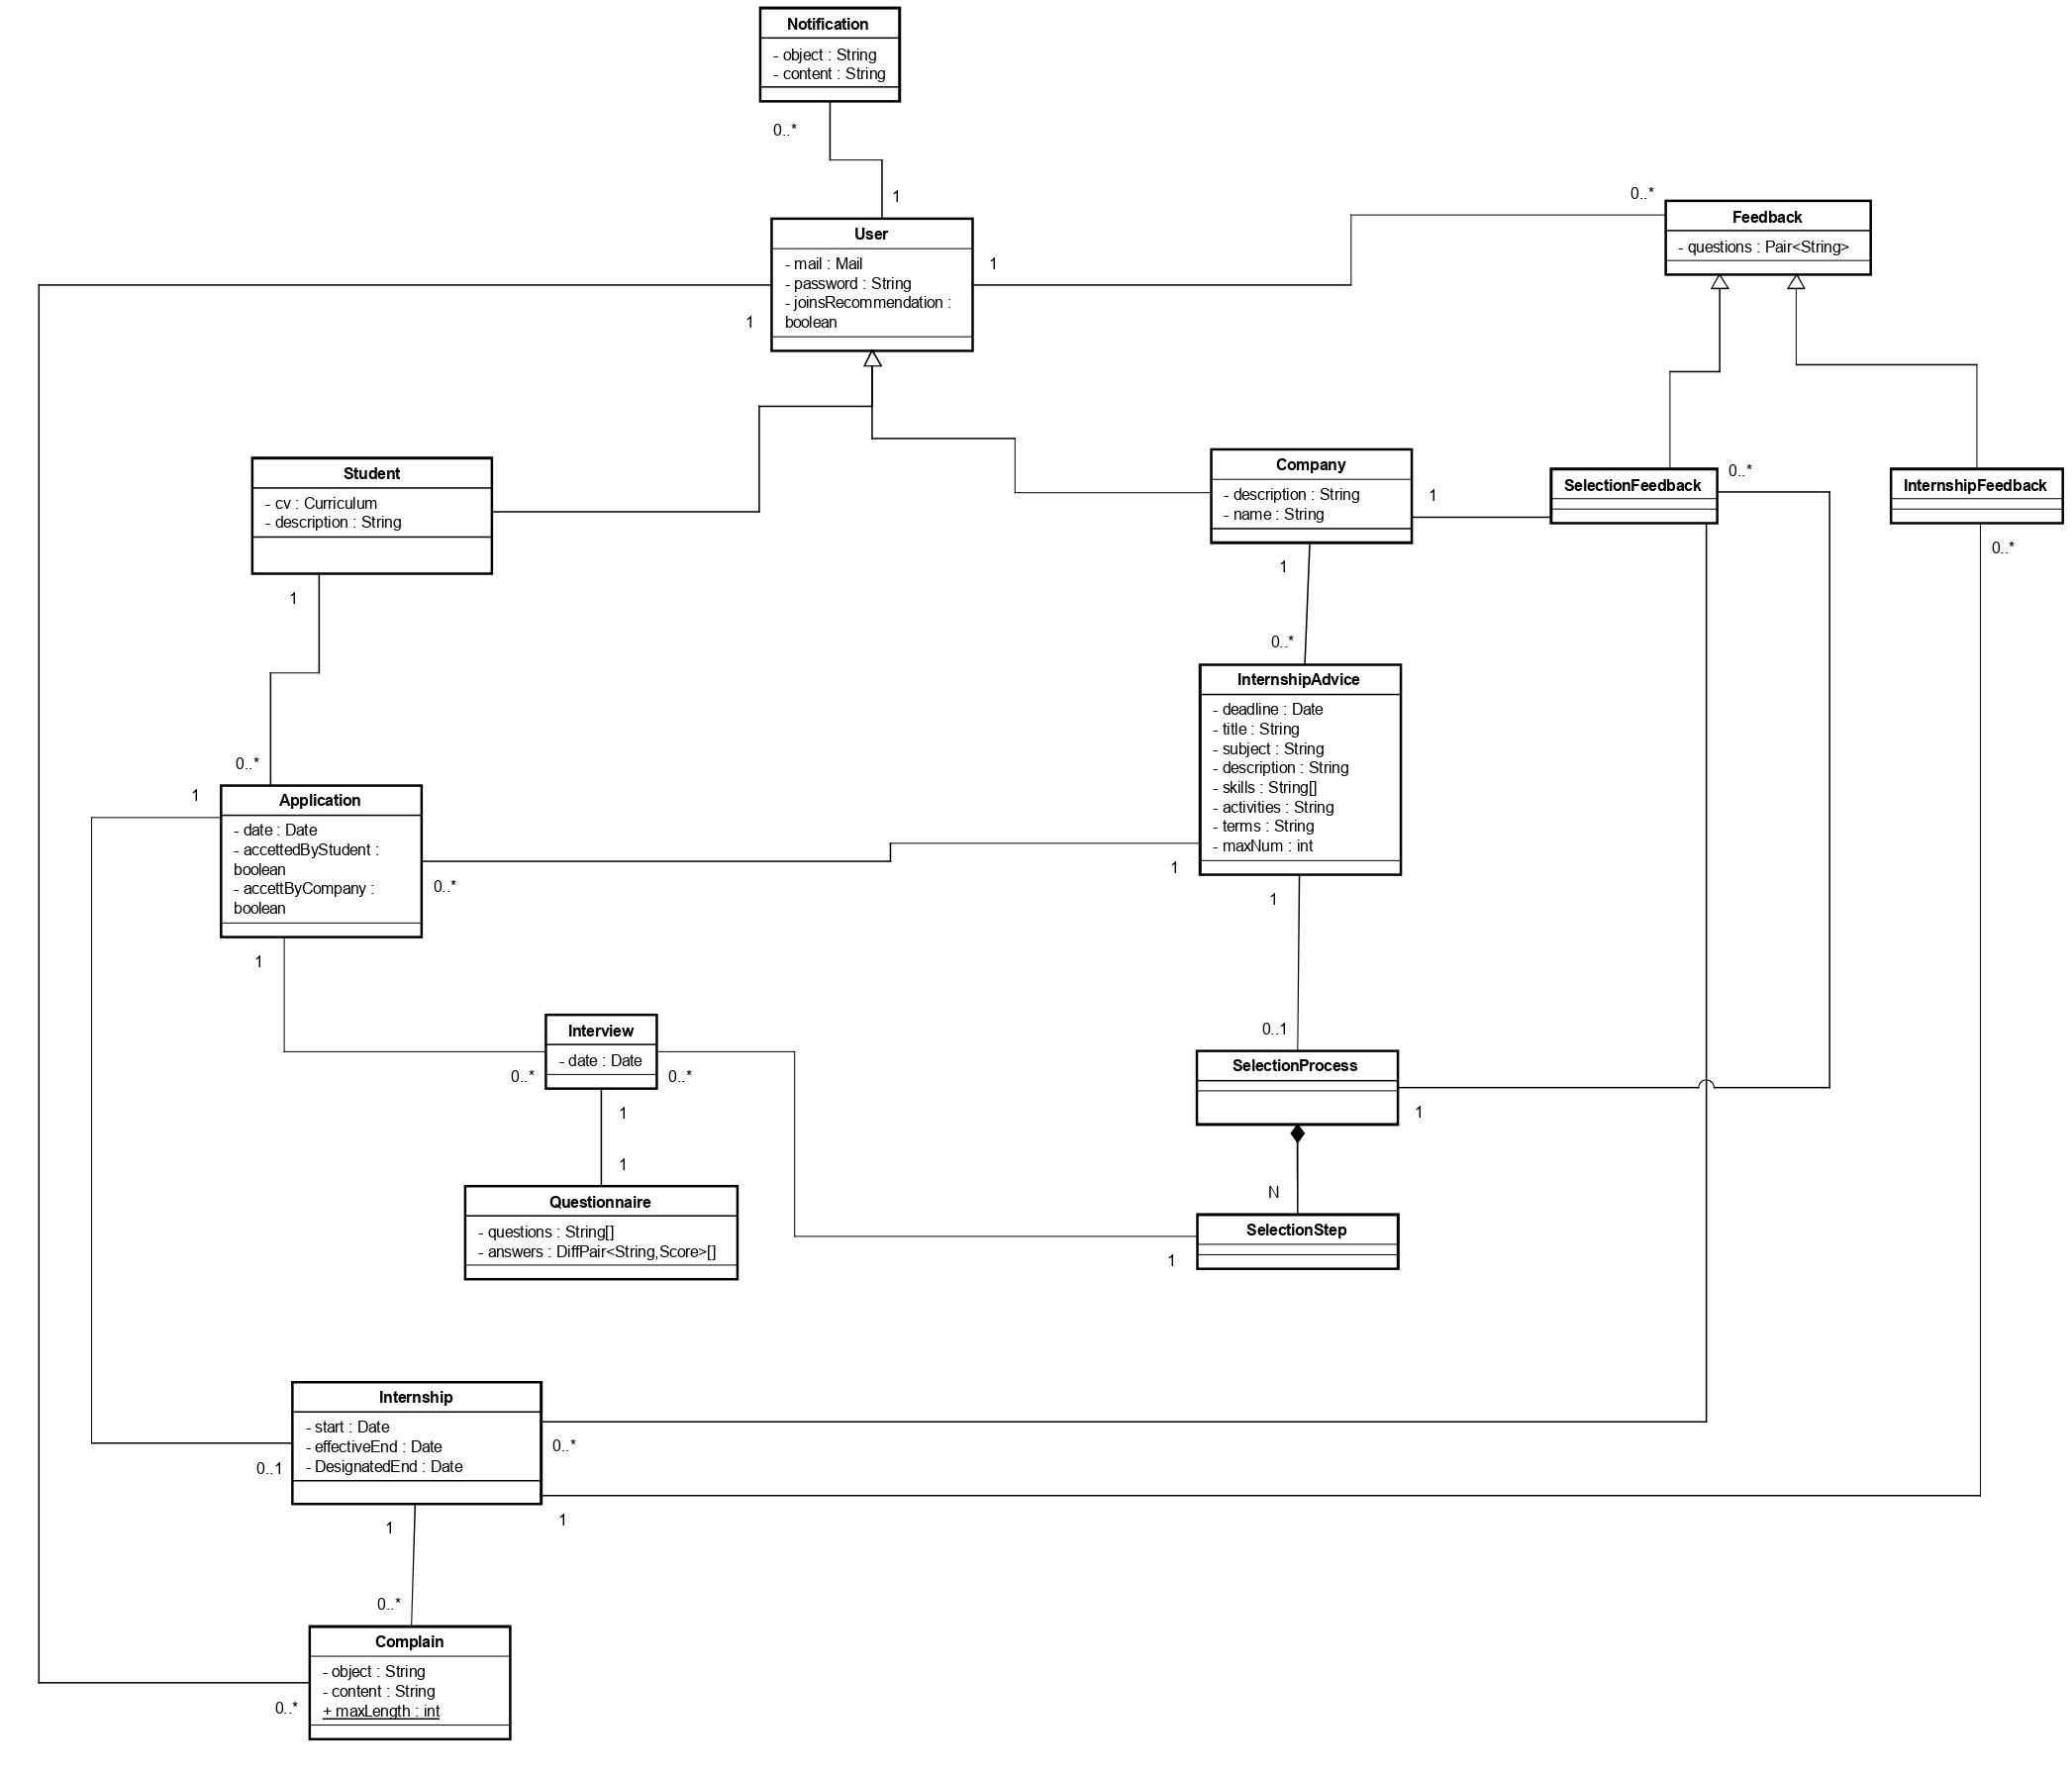
\includegraphics{CLASS DIAGRAM (NO NOT).jpg}
			
			This figure represent the domain class diagram of the system. It represents the fact that the system connects students and companies, facilitating the management of applications, selection processes, interviews, internships, and communication between the parties. It provides tools for sending notifications, collecting feedback, and managing questionnaire and complaints.
			
			The system's users are modeled through the \textit{User} class, which represents both Students (class \textit{Student}) and Companies (class \textit{Company}). Each user has basic attributes (email and password) and can receive personalized notifications (class \textit{Notification}, with subtypes for students and companies).
			
			Companies can publish internships advice (class \textit{InternshipAdvice}); students can apply for an internship but also companies can send proposal of application to the students. This mechanism of applications is managed by the \textit{Application} class. Each application born with one and only one of the boolean flags to true, corresponding to the kind of user that unleashed that application. Once the other user accepts the proposal of the counterpart, its flag is put to \textit{true}; at the end, students that will enroll the selection process are the only related to applications with the 2 flags true.
			
			Each application can go through a \textit{SelectionProcess}, divided into several \textit{SelectionStep}. During the selection process, the student may undergo an interview (\textit{Interview} class) and his answers are collected by the system through questionnaires (\textit{Questionnaire} class).
			
			Internship advice is associated with a concrete Internsihp (class \textit{Internship}) offered by companies; Internships are linked to feedback (\textit{InternshipFeedback}) and complaints (\textit{Complain}). 
			The system supports the collection of feedback in two forms:
			\begin{itemize}
				\item \textit{SelectionFeedback}: feedback on the selection processes.
				\item {InternshipFeedback}: feedback related to internships
			
			\end{itemize}
			
			
			
			
			
			
			
			
			
			\subsection{State Diagrams}
				In this subsection, the most relevant state diagrams are presented in order to better understand the system's evolution through its different phases. We focus in particular on the representation of an internship's state and the evolution of a student's application.
				
				\subparagraph{State of an internship}
					\begin{center}
						\includegraphics[scale=0.3]{stateInternship.jpg}
					\end{center}
					
					In this state diagram, each state represents the status an internship can have. \textit{Activated} is the state where the internship is published and visible on the platform (in the form of an internship advice); \textit{Under Selection} is the state where the company is conducting the selection process;\textit{Assigned} is the state where the internship has been assigned to specific students; \textit{Closed} is the state where the internship has ended (either because it finished or was interrupted); \textit{Deleted} is the state where the internship is removed from the system (the company deletes the internship advice or the selection process is ended).
					
				\subparagraph{State of an application for an internship}
					\begin{center}
						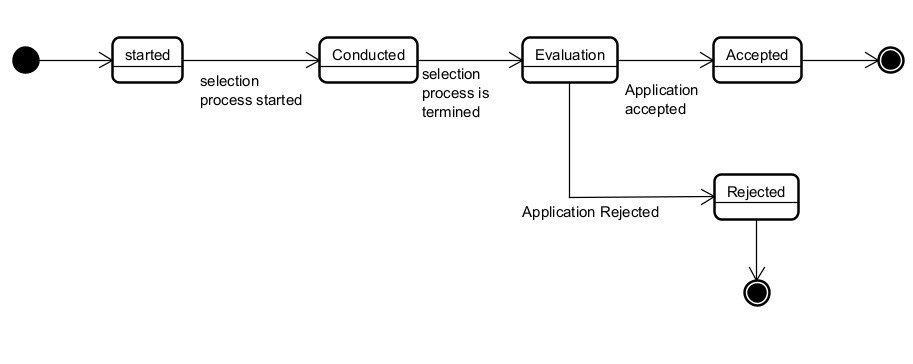
\includegraphics[scale=0.3]{application.jpg}
					\end{center}
					
					In this state diagram, the evolution of a student's application for an internship is described. The \textit{Started} state refers to a student's application for an internship. The \textit{Conducted} state relates to the evolution of the selection process (open questions, closed questions, interviews, questionnaire completion, etc.). The \textit{Evaluation} state is where the company assesses the student's application. From this state, two subsequent states are possible: \textit{Accepted} if the application is accepted, or \textit{Rejected} if it is declined.
					
	\section{Product functions}
		\textbf{Sign-up and login}
			\begin{flushleft}
				This functionality permits to both students and companies to set up their personal profile on the platform and accessing to the latter via their personal information (e-mail and password). Students profiles specify basic information regarding students interests and include their CV while companies profile include all the information that may help student in understanding companies vision and business area.
			\end{flushleft}
		\textbf{Internship proposal management}
			\begin{flushleft}
				Companies can post advice for internship they are going to offer and students can proactively search for them. In this case, a student that wants to apply for an internship sends a request to the company and it decides or not to enroll the student into the selection process. Moreover, thanks to the recommendation feature, companies receives profiles of possibly interested students and students receive profiles of companies that offer internship possibly related to their interests. Therefore, a companies can also suggest to a student to apply for an internship selection and students can accept or decline this proposal.
			\end{flushleft}
		\textbf{Recommendation mechanism}
			\begin{flushleft}
				This functionality aims to facilitate the establishment of a contact between students and companies. By means of recommendation analysis, the system is able to propose to students internships advice that may interest them and to companies students that may be interested to their internships. This analysis are supported by companies and students profiles (CVs in particular, for students) and not compulsory feedback collected at the end of selections processes or internships.
			\end{flushleft}
		\textbf{Selection process management}
			\begin{flushleft}
				A selection process can be supported by the system from the advice deadline to its finalization. In particular, companies can use the system to define process steps, schedule interviews, correct closed questions and compare students results each other (by defining their metrics).
			\end{flushleft}
		\textbf{Internship monitoring}
			\begin{flushleft}
				Students that are currently involved in active internships can use the system to post complains and monitor the current status of them. On the other side, also companies can also post complains on internships they are currently providing (and of course they can also monitor their status).
			\end{flushleft}
		\textbf{Notifications management}
			\begin{flushleft}
				Each message that is sent to companies or students (e.g. selection results, internship proposal, interview dates) are also sent to profile e-mail addresses (a short version of them). From the system, each message can be read entirely.
			\end{flushleft}
	\section{User characteristics}
		there are mainly two types of user that interact with the platform: Student and Companies.
		\subsection{Student}
			The student, once logged into the platform, is able to proactively search for internship advice that may interest them. Once the internship of interest has been selected, they can apply for an interview directly through the platform. Additionally, the student receives a list of possible internships that may suit them, based on their studies/CV, via the aforementioned recommendation mechanism. Furthermore, the student may also receive a proposal to apply directly from the company offering the internship. Once they have completed a selection process, the student will receive the outcome directly through the platform.
		
		\subsection{Company}
			The company, once logged into the platform, can publish internship announcements it wants to offer. The system will periodically send the company a list of potential students who may be suitable for their internships, based on their CVs, to whom it can directly send a proposal to apply for one of its internships. Conversely, the company can also accept or reject a student's application. For a given internship, once the application period has ended, the company can schedule the selection process for each candidate directly through the system. During the selection phase, the company also collects all candidate responses using the system.Finally, the company will provide the outcome of the selection to each student directly through the platform.
		
		\subsection{common characteristics}
			Both users can also provide feedback on the selection process as well as at the end of the internship. This feedback is collected by the system to improve the recommendation process. Additionally, both users can monitor the status of an outgoing internship and provide information or complaints about it.
		
	\section{Assumptions, dependencies and constraints}
		\subsection{Domain Assumption}
			the following assumption are made for domain. They are properties or condition that the system will take for granted. They must be checked to ensure a correct platform behavior.
			
			[D1] Users must have a reliable internet connection
			
			[D2] Information contained in the CVs are truthful
			
			[D3] Company fill the form about internship advice accordingly to their business decisions
			
			[D4] Company correctly enters the answers provided by the student during the interview into the system
			
			[D5] When users registers, they register with an active email address that belongs to them
			
			[D6] Uploaded CVs are written in EuroPass format
			
			[D7] Information on a student CV do not contradict each other
			
			[D8] Information companies insert in internship advice do not contradict each other
			
		\subsection{Dependencies}
			\begin{itemize}
				\item The system will integrate with email system to send notifications to Users
			\end{itemize}
		
		\subsection{Constraints}
			\begin{itemize}
				\item The system shall be compliant to local laws and regulations, in particular users data should be treated
				according to the GDPR. This means that users should be always able to request their data
				\item The data collected for matching (feedback, ...) are sufficiently detailed to support effective statistical analysis.
				\item The number of students and companies using the platform will be manageable by the system without compromising its performance
				\item To better protect the users’ sensitive information their data should be encrypted
			\end{itemize}
		
%Considerazioni:
%	i requirements sono stati scritti con questa idea:
%	una compagnia può “proporre” una internship a uno studente 	(manca uno scenario per questo, potrebbe essere aggiunto a quello della notifica). Si veda il requirement “R10602”
%	non ho modellizzato il concetto di “richiesta di candidatura” (ma uno si candida e basta). Se non sei d’accordo lo metto.
% mettere nelle definizioni la differenza tra internship e internship advice

% METTERE SCREMATURA INIZIALE BASATA SUL CURRICULUM E METTERE MAX POSTI PER UN ADVICE (SE IL MAX POSTI E' RAGGIUNTO L'ADVICE E' ANCORA VISIBILE MA NON CI SI PUO' CANDIDARE) [MODIFICARE QUESTE COSE NEI REQ. E NELL'ALLOY]

% RIGUARDARE LA SPECIFICA PER QUANTO RIGUARDA I FEEDBACK E I COMPLAINT (E ANCHE IL FATTO CHE "INTERNSHIP" NEL CLASS DIAGRAM NON E' "LA MIA INTERNSHIP" MA LA INTERNSHIP IN GENERALE, MAGARI NON E' UN ERRORE MA DI QUESTA COSA VA TENUTO CONTO)

% RIGUARDARE I REQ. PER LE NOTIFICHE (TUTTE, ANHE QUELLE LEGATE ALL'ESITO DELLA SELEZIONE)

% ENTITA' "NOTIFICA" NEL CLASS DIAGRAM?
\chapter{Specific requirements}
	\section{External Interface Requirements}
		\subsection{User Interfaces}
		\subsection{Hardware Interfaces}
		\subsection{Software Interfaces}
		\subsection{Communication Interfaces}
	\section{Functional Requirements}
		\subsection{Use-case diagrams}
		\subsection{Use-cases}
		\subsection{Sequence diagrams}
		\subsection{Activity diagrams}
		\subsection{Requirements mapping}
			\begin{table} [h!]
				\centering
				\begin{tabular}{ || P{7.5cm} P{7.5cm} || }
					\hline
						\multicolumn{2}{||P{15cm}||}{[G1] students and companies establish contacts for doing internships} \\ [0.5ex]
					\hline
					[R10101] the system allows students to sign up to the platform with their institutional mails & [D10101] students upload their CV in Europass format \\
					
					[R10102] the system allows a student to set up whether he/she wants to be notified of the presence of internship advice that might interest him/her & [D10102] information on a student CV do not contradict each other \\
					
					[R10103] the system allows students upload their CV to the platform & [D10302] information companies insert in internship advice do not contradict each other \\
					
					[R10104] the system allows students to publish on their profile a brief description of themselves & \\
					
					[R10201] the system allows companies to sign up to the platform with their company address & \\
					
					[R10202] the system allows companies to insert the main information regarding their business area and area of expertise & \\
					
					[R10203] the system allows a company to set up whether it wants to be notified of the presence of students that might be interested to its internship advice & \\
					
					[R10301] the system allows companies to publish internship advice where they specify the main information regarding the internship (brief description, experience required, desired skills, main activities involved and the terms) and the submission deadline & \\
					
					[R10401] the system allows students to search internships advice by name (and also to see the complete list of available advice). The system shall act as a search engine to present also the names of the advice that are similar to the searched one & \\
					
					[R10402] the system allows students to search companies by name (and also to see the complete list of registered companies) and then access to their profile & \\
					
					[R10403] the system allows students to filter the results they searched (e.g. "only paid internships", "only companies located in Lombardy") & \\
					
					[R10501] when the system recognizes that a new internship advice that might interest a student (that allowed the notification option) is published it notifies that student by sending him an e-mail (to your address) & \\
					
					[R10601] when the system recognizes that a student has a profile that would fit an internship advice, the company that published the advice is notified & \\
					
					[R10602] when a company opens a student profile, it can propose to him to apply for one of its internships & \\
					
					[R10701] the system allows students to apply for any internship advice which deadline has not expired & \\
					
					[R10702] when a student applies for an internship, the related company is notified by the system & \\ [1ex]
					\hline
				\end{tabular}
				\caption{Requirements mapping for goal G1}
				\label {table:1}
			\end{table}
			\begin{table} [h!]
				\centering
				\begin{tabular}{ || P{7.5cm} P{7.5cm} || }
					\hline
					\multicolumn{2}{||P{15cm}||}{[G2] internships selections can be monitored and supported by the system} \\ [0.5ex]
					\hline
					[R20101] when the deadline for an internship advice is expired, the system allows the company to set up the selection process by specifying for each step, the relative questionnaire (with metrics for each question) and the date in which provide it to a student (dates may differ between different students) & \\
					
					[R20201] the system automatically calculates the scores of questionnaire closed answers & \\
					
					[R20202] the system allows companies to manually insert scores for questionnaire open answers & \\
					
					[R20203] the system allows companies to visualize and compare selections scores & \\
					
					[R20204] in any selection phase, the system allows companies to discard a student currently involved in the selection process (discarded students are removed by the selection process) & \\
					
					[R20205] in any selection phase, the system allows companies to accept a student currently involved in the selection process (accepted students are removed by the selection process) & \\
					
					[R20206] the system allows companies to write a personalized message to communicate the result of a selection & \\ [1ex]
					\hline
				\end{tabular}
				\caption{Requirements mapping for goal G2}
				\label {table:1}
			\end{table}
			\begin{table} [h!]
				\centering
				\begin{tabular}{ || P{7.5cm} P{7.5cm} || }
					\hline
					\multicolumn{2}{||P{15cm}||}{[G3] ongoing internships can be monitored from the system} \\ [0.5ex]
					\hline
					[R30101] the system allows students and companies to consult the internships (ongoing or finished) & \\
					
					[R30102] the system allows students and companies to report complaints on the internships they are involved in & \\ [1ex]
					\hline
				\end{tabular}
				\caption{Requirements mapping for goal G3}
				\label {table:1}
			\end{table}
	\section{Performance Requirements}
	\section{Design Constraints}
		\subsection{Standards compliance}
		\subsection{Hardware limitations}
		\subsection{Other constraints}
	\section{Software System Attributes}
		\subsection{Reliability}
		\subsection{Availability}
		\subsection{Security}
		\subsection{Maintainability}
		\subsection{Portability}
\setchapterimage[7.5cm]{seaside}
%\chapter[Figures and Tables]{Figures and Tables\footnotemark[0]}
\chapter{Figures and Tables}

\footnotetext{The credits for the image above the chapter title go to:
	Bushra Feroz, CC~BY-SA~4.0, \url{https://commons.wikimedia.org/w/index.php?curid=68724647}}

\section{Normal Figures and Tables}

Figures and tables can be inserted just like in any standard 
\LaTeX\xspace document. The \Package{graphicx} package is already loaded 
and configured in such a way that the figure width is equal to the 
textwidth and the height is adjusted in order to maintain the original 
aspect ratio. As you may have imagined, the captions will be 
positioned\ldots well, in the margins. This is achieved with the help of 
the \Package{floatrow} package.

Here is a picture of Mona Lisa (\reffig{normalmonalisa}), as an example. 
The captions are formatted as the margin- and the side-notes; If you 
want to change something about captions you can use the command 
\Command{captsetup} from the \Package{caption} package. Remember that if 
you want to reference a figure, the label must come \emph{after} the 
caption!

\begin{figure}[hb]
	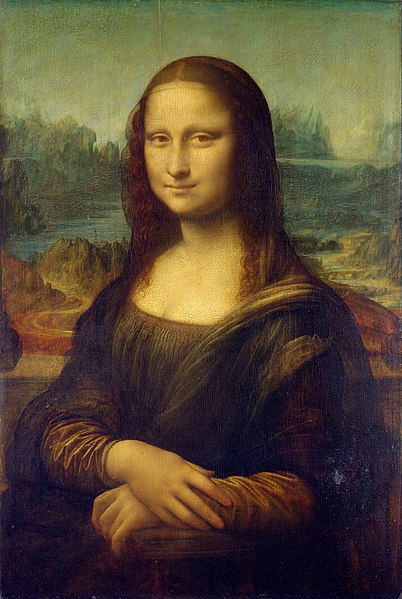
\includegraphics[width=0.45\textwidth]{monalisa}
	\caption[Mona Lisa, again]{It's Mona Lisa again. \blindtext}
	\labfig{normalmonalisa}
\end{figure}

While the format of the caption is managed by \Package{caption}, its 
position is handled by the \Package{floatrow} package. Achieving this 
result has been quite hard, but now I am pretty satisfied. In two-side 
mode, the captions are printed in the correct margin.

Tables can be inserted just as easily as figures, as exemplified by the 
following code:

\begin{lstlisting}[caption={Caption of a listing.}]
\begin{table}
\begin{tabular}{ c c c c }
	\toprule
	col1 & col2 & col3 & col 4 \\
	\midrule
	\multirow{3}{4em}{Multiple row} & cell2 & cell3 & cell4\\ &
	cell5 & cell6 & cell7 \\ &
	cell8 & cell9 & cell10 \\
	\multirow{3}{4em}{Multiple row} & cell2 & cell3 & cell4 \\ &
	cell5 & cell6 & cell7 \\ &
	cell8 & cell9 & cell10 \\
	\bottomrule
\end{tabular}
\end{table}
\end{lstlisting}

which results in the useless \vreftab{useless}.

\begin{table}[ht]
\caption[A useless table]{A useless table.}
\labtab{useless}
\begin{tabular}{ c c c c }
	\toprule
	col1 & col2 & col3 & col 4 \\
	\midrule
	\multirow{3}{4em}{Multiple row} & cell2 & cell3 & cell4\\ &
	cell5 & cell6 & cell7 \\ &
	cell8 & cell9 & cell10 \\
	\multirow{3}{4em}{Multiple row} & cell2 & cell3 & cell4 \\ &
	cell5 & cell6 & cell7 \\ &
	cell8 & cell9 & cell10 \\
	\bottomrule
\end{tabular}
\end{table}

I don't have much else to say, so I will just insert some blind text. 
\blindtext

\section{Margin Figures and Tables}

Marginfigures can be inserted with the environment 
\Environment{marginfigure}. In this case, the whole picture is confined 
to the margin and the caption is below it. \reffig{marginmonalisa} is 
obtained with something like this:

\begin{lstlisting}[caption={Another caption.}]
\begin{marginfigure}
	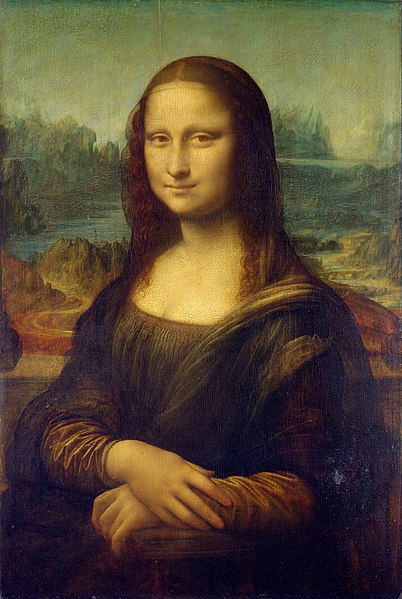
\includegraphics{monalisa}
	\caption[The Mona Lisa]{The Mona Lisa.}
	\labfig{marginmonalisa}
\end{marginfigure}
\end{lstlisting}

There is also the \Environment{margintable} environment, of which 
\reftab{anotheruseless} is an example. Notice how you can place the 
caption above the table by just placing the \Command{caption} command 
before beginning the \Environment{tabular} environment. Usually, figure 
captions are below, while table captions are above. This rule is also 
respected for normal figures and tables: the captions are always on the 
side, but for figure they are aligned to the bottom, while for tables to 
the top.

\begin{margintable}
\caption[Another useless table]{Another useless table.}
\labtab{anotheruseless}
\raggedright
\begin{tabular}{ c c c c }
	\hline
	col1 & col2 & col3 \\
	\hline
	\multirow{3}{4em}{Multiple row} & cell2 & cell3 \\ & cell5 & cell6 
	\\ & cell8 & cell9 \\ \hline
\end{tabular}
\end{margintable}

Marginfigures and tables can be positioned with an optional offset 
command, like so:

\begin{lstlisting}
\begin{marginfigure}[offset]
	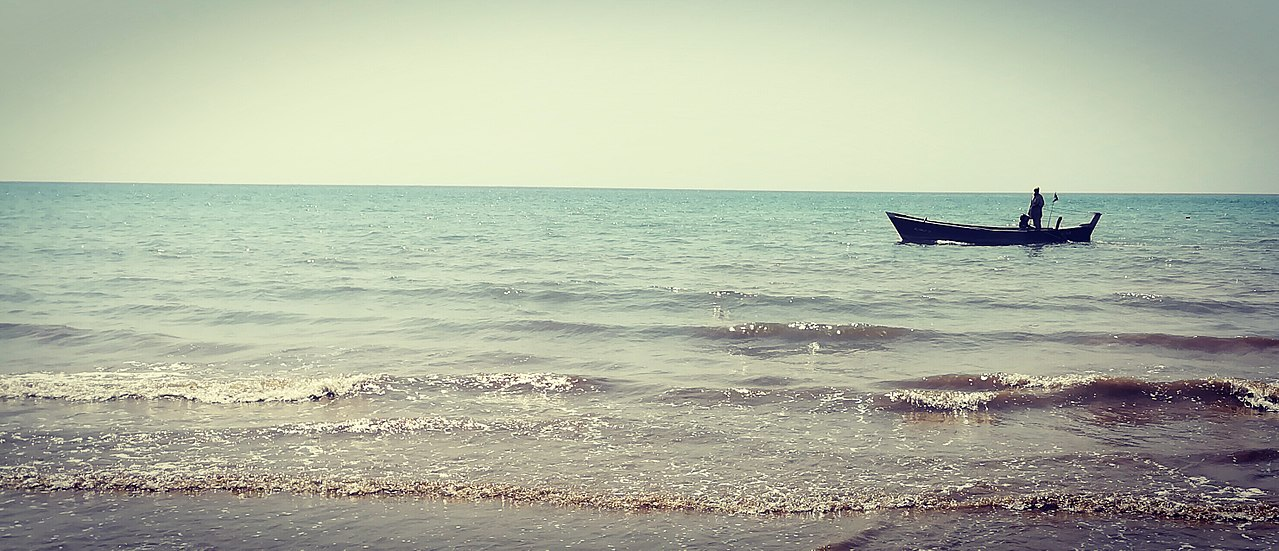
\includegraphics{seaside}
\end{marginfigure}
\end{lstlisting}

Offset ca be either a measure or a multiple of \Command{baselineskip}, 
much like with \Command{sidenote}, \Command{marginnote} and 
\Command{margintoc}.\todo{Improve this part.} If you are wondering how I 
inserted this orange bubble, have a look at the \Package{todo} package.

\section{Wide Figures and Tables}

With the environments \Environment{figure*} and \Environment{table*} you 
can insert figures which span the whole page width. For example, here 
are a wide figure and a wide table.

\begin{figure*}[h!]
	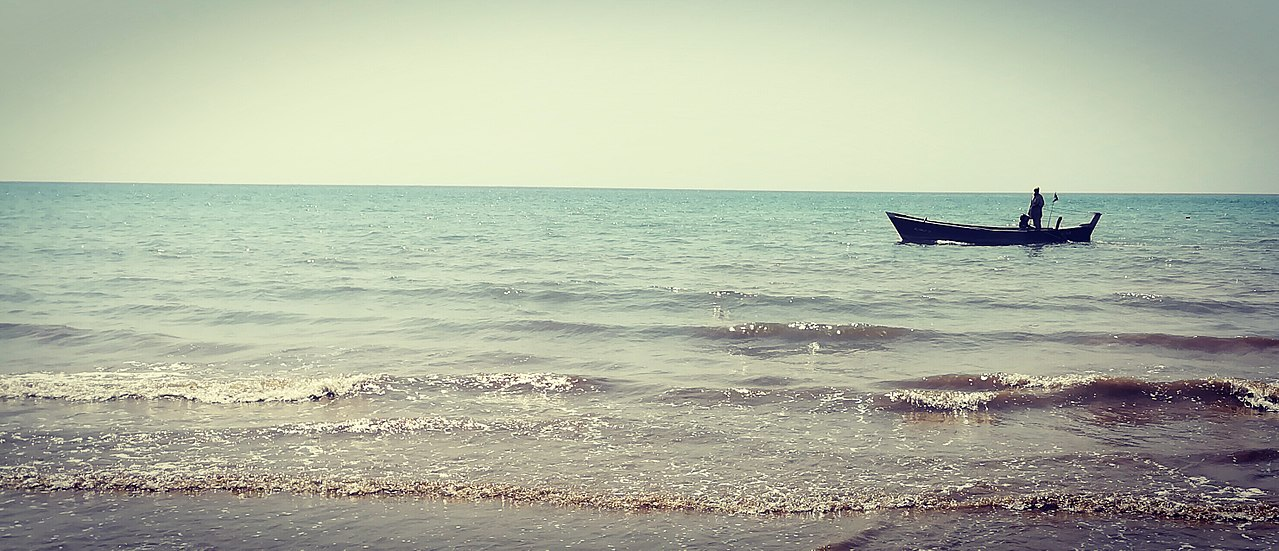
\includegraphics{seaside}
	\caption[A wide seaside]{A wide seaside, and a wide caption.
		Credits: By Bushra Feroz, CC BY-SA 4.0, \url{https://commons.wikimedia.org/w/index.php?curid=68724647}}
\end{figure*}

\begin{table*}[h!]
    \caption{A wide table with invented data about three people living in the UK. Note that wide figures and tables are centered and their caption also extends into the margin.}
    \begin{tabular}{p{2.0cm} p{2.0cm} p{2.0cm} p{2.0cm} p{2.0cm} p{2.0cm} p{1.5cm}}
        \toprule
        Name    & Surname   & Job       & Salary           & Age   & Height    & Country \\
        \midrule
        Alice   & Red       & Writer    & 4.000 \pounds    & 34    & 167 cm     & England \\
        Bob     & White     & Bartender & 2.000 \pounds    & 24    & 180 cm     & Scotland \\
        Drake   & Green     & Scientist & 4.000 \pounds    & 26    & 175 cm     & Wales \\
        \bottomrule
    \end{tabular}
\end{table*}

It is the user's responsibility to adjust the width of the table, if 
necessary, until it is aesthetically pleasing. The previous table was 
obtained with the following code:

\begin{lstlisting}[caption=How to typeset a wide table]
\begin{table*}[h!]
    \caption{A wide table with invented data about three people living in the UK. Note that wide figures and tables are centered and their caption also extends into the margin.}
    \begin{tabular}{p{2.0cm} p{2.0cm} p{2.0cm} p{2.0cm} p{2.0cm} p{2.0cm} p{1.5cm}}
        \toprule
        Name    & Surname   & Job       & Salary           & Age   & Height    & Country \\
        \midrule
        Alice   & Red       & Writer    & 4.000 \pounds    & 34    & 167 cm     & England \\
        Bob     & White     & Bartender & 2.000 \pounds    & 24    & 180 cm     & Scotland \\
        Drake   & Green     & Scientist & 4.000 \pounds    & 26    & 175 cm     & Wales \\
        \bottomrule
    \end{tabular}
\end{table*}
\end{lstlisting}

The \Package{floatrow} package provides the \enquote{H} specifier to 
instruct \LaTeX to position the figure (or table) in precisely the same 
position it occupies in the source code. However, this specifier does 
not work with wide figures or tables: you should use \enquote{h!} 
instead, like so: \lstinline|\begin{figure*}[h!]|.

You may have noticed the full width image at the very beginning of this
chapter: that, however, is set up in an entirely different way, which
you'll read about in \vrefch{layout}.

\Class{kaobook} also supports paginated tables (have a look at the 
\Package{longtable} package). The 
\Environment{longtable}\sidenote{Interestingly, \Environment{longtable}s 
may require up to four rounds of compilation before they are typeset 
correctly.} environment behaves a bit differently from 
\Environment{table}, in that \Environment{longtable} encompasses both 
\Environment{table} and \Environment{tabular}, so that you can write, 
\eg,

\begin{lstlisting}[caption=Example of a longtable]
\begin{longtable}{|l c c|}
    \hline
    One & Two & Three \\
    Left & Center & Center \\
    \hline
    \caption{Caption of the longtable.}
\end{longtable}
\end{lstlisting}

to obtain the following table:
\begin{longtable}{|l c c|}
    \hline
    One & Two & Three \\
    Left & Center & Center \\
    \hline
    \caption{Caption of the longtable.}
\end{longtable}

The caption of a \Environment{longtable} is always positioned below the 
table, and it has the same width as the text (it doesn't extend into the 
margin). However, sometimes you may need a \Environment{longtable} that 
is so wide that it trespass into the margins; in those cases, you may 
want to also increase the width of the caption. To do so, you'll have to 
write two additional commands, one before and one after the 
\Environment{longtable}:

\begin{lstlisting}[caption=Increasing the width of the caption of a \Environment{longtable}.]
\floatsetup[longtable]{margins=centering,LTcapwidth=table} % Add this line before the longtable to increase the caption width
\begin{longtable}{lp{8cm}p{5cm}p{2cm}}
...
\end{longtable}
\floatsetup[longtable]{margins=raggedright,LTcapwidth=\textwidth} % Add this line after the longtable to revert the previous change
\end{lstlisting}

Having seen figures and tables, it is now time to tackle 
hyperreferences.

\chapter{Effort Spent}
	\begin{center}
		\begin{table}[H]
			\begin{tabular}{ | m{3.2cm} | m{1cm}| m{4cm} | m{1.5cm}| m{4cm} | } 
				\hline
					&  \multicolumn{2}{c|}{ Andrea} & \multicolumn{2}{c|}{ Alessandro} \\ 
				\hline
					\textbf{Week} & \textbf{Hours}   & \textbf{Category} & \textbf{Hours}       & \textbf{Category} \\
				\hline
					21/10/2024 - 27/10/2024 & 6 & Resume course notes and assignment analysis & 3 & Assignment analysis\\
				\hline
					28/10/2024 - 03/11/2024 & 0.5 & First goal definition & 2.5 & Deeper assignment analysis and first scenarios \\
				\hline
					04/11/2024 - 10/11/2024 & 1.5 & First requirements definition and first high-level class diagram & 3 & RASD introduction and first phenomena definition\\
				\hline
					11/11/2024 - 17/11/2024 & 0 & - & 2 & Deeper scenarios definition \\
				\hline
					18/11/2024 - 24/11/2024 & 12 & First Alloy modeling, requirements deeper analysis, selection process scenarios & 4 & Phenomena deeper analysis, scenarios adjustments\\
				\hline
					25/11/2024 - 01/12/2024 & 1.5 & Requirements and class diagram adjustments & 3 & Use-case initial definition \\
				\hline
					02/12/2024 - 08/12/2024 & 2 & Scenarios and requirements completion and non-functional requirements definition & 4 & Use-case deeper definition and non-functional requirements definition\\
				\hline
					09/12/2024 - 15/12/2024 & 8 & Alloy completion and product-functions & 6 & Use-cases completion, sequence and state diagrams definition\\
				\hline
					16/12/2024 - 22/12/2024 & 5 & Final overview, Effort Spent compilation and User Interfaces & 9 & Final overview and Sequence, state, activity, use-case diagrams completion and User Interfaces\\
				\hline
					\textbf{TOTAL} & \textbf{36.5} & & \textbf{36.5} & \\
				\hline
			\end{tabular}
			\caption{Effort spent overview}
		\end{table}
	\end{center}

\pagelayout{wide} % No margins
\addpart{Design and Additional Features}


\chapter{Software Used}
\begin{center}
	\begin{table}[H]
		\begin{tabular}{ | m{3cm} | m{3cm} | m{3cm} | } 
			\hline
			\textbf {Software} & \textbf{Version} & \textbf{Usage} \\
			\hline
			TeXstudio & 4.6.3 & Writing Latex \\
			\hline
			PdfLaTeX & - & Latex compilation \\
			\hline
			XeLaTex & - & Latex compilation \\
			\hline
			Astah UML & 9.2.0/0248cd & UML diagrams \\
			\hline
			Alloy Analyzer & 6.1.0 & Alloy modeling \\
			\hline
			miro.com & - & User interface maps and mock-up, high-level view, logic scheme \\
			\hline
			draw.io & - & Component view, deployment view \\
			\hline
		\end{tabular}
		\caption{Software used overview}
	\end{table}
\end{center}

This document was written over the template kaobook designed by Federico Marotta (\url{https://github.com/fmarotta/kaobook}), with few adjustments by us.
\chapter{Effort Spent}
\begin{center}
	\begin{table}[H]
		\begin{tabular}{ | m{3.2cm} | m{1cm}| m{4cm} | m{1.5cm}| m{4cm} | } 
			\hline
			&  \multicolumn{2}{c|}{ Andrea} & \multicolumn{2}{c|}{ Alessandro} \\ 
			\hline
			\textbf{Week} & \textbf{Hours}   & \textbf{Category} & \textbf{Hours}       & \textbf{Category} \\
			\hline
			23/12/2024 - 29/12/2024 & 16 & User interface and high-level structure & 4 & high-level structure\\
			\hline
			30/12/2024 - 05/01/2025 & 2 & Data logic model & 12 & Introduction, data logic model, sequence diagrams\\
			\hline
			06/01/2025 - 07/01/2025 & 8 & Final revision, requirements mapping, integration and test plan, component view, deployment view, effort spent and software used compilation & 6 & Final revision, requirements mapping, integration and test plan, component view\\
			\hline
			\textbf{TOTAL} & \textbf{26} & & \textbf{22} & \\
			\hline
		\end{tabular}
		\caption{Effort spent overview}
	\end{table}
\end{center}

\appendix % From here onwards, chapters are numbered with letters, as is the appendix convention

\pagelayout{wide} % No margins
\addpart{Appendix}


\setchapterstyle{lines}
\labch{appendix}
\blinddocument

\chapter{Fonts Testing}

\section{Font Sizes}

{\tiny The quick brown fox jumps over the lazy dog.}

{\scriptsize The quick brown fox jumps over the lazy dog.}

{\footnotesize The quick brown fox jumps over the lazy dog.}

{\small The quick brown fox jumps over the lazy dog.}

{\normalsize The quick brown fox jumps over the lazy dog.}

{\large The quick brown fox jumps over the lazy dog.}

{\Large The quick brown fox jumps over the lazy dog.}

{\LARGE The quick brown fox jumps over the lazy dog.}

{\huge The quick brown fox jumps over the lazy dog.}

{\Huge The quick brown fox jumps over the lazy dog.}


\section{Font Families}

\sffamily\blindtext

\textmd{The quick brown fox jumps over the lazy dog. Medium.}

\textbf{The quick brown fox jumps over the lazy dog. Bold.}

\textup{The quick brown fox jumps over the lazy dog. Upright.}

\textit{The quick brown fox jumps over the lazy dog. Italics.}

\textsl{The quick brown fox jumps over the lazy dog. Slanted.}

\textsc{The quick brown fox jumps over the lazy dog. Small Caps.}

\ttfamily\blindtext

\textmd{The quick brown fox jumps over the lazy dog. Medium.}

\textbf{The quick brown fox jumps over the lazy dog. Bold.}

\textup{The quick brown fox jumps over the lazy dog. Upright.}

\textit{The quick brown fox jumps over the lazy dog. Italics.}

\textsl{The quick brown fox jumps over the lazy dog. Slanted.}

\textsc{The quick brown fox jumps over the lazy dog. Small Caps.}

\rmfamily\blindtext

\textmd{The quick brown fox jumps over the lazy dog. Medium.}

\textbf{The quick brown fox jumps over the lazy dog. Bold.}

\textup{The quick brown fox jumps over the lazy dog. Upright.}

\textit{The quick brown fox jumps over the lazy dog. Italics.}

\textsl{The quick brown fox jumps over the lazy dog. Slanted.}

\textsc{The quick brown fox jumps over the lazy dog. Small Caps.}



%----------------------------------------------------------------------------------------

\backmatter % Denotes the end of the main document content
\setchapterstyle{plain} % Output plain chapters from this point onwards

%----------------------------------------------------------------------------------------
%	BIBLIOGRAPHY
%----------------------------------------------------------------------------------------

% The bibliography needs to be compiled with biber using your LaTeX editor, or on the command line with 'biber main' from the template directory

\defbibnote{bibnote}{Here are the references in citation order.\par\bigskip} % Prepend this text to the bibliography
\printbibliography[heading=bibintoc, title=Bibliography, prenote=bibnote] % Add the bibliography heading to the ToC, set the title of the bibliography and output the bibliography note

%----------------------------------------------------------------------------------------
%	NOMENCLATURE
%----------------------------------------------------------------------------------------

% The nomenclature needs to be compiled on the command line with 'makeindex main.nlo -s nomencl.ist -o main.nls' from the template directory

\nomenclature{$c$}{Speed of light in a vacuum inertial frame}
\nomenclature{$h$}{Planck constant}

\renewcommand{\nomname}{Notation} % Rename the default 'Nomenclature'
\renewcommand{\nompreamble}{The next list describes several symbols that will be later used within the body of the document.} % Prepend this text to the nomenclature

\printnomenclature % Output the nomenclature

%----------------------------------------------------------------------------------------
%	GREEK ALPHABET
% 	Originally from https://gitlab.com/jim.hefferon/linear-algebra
%----------------------------------------------------------------------------------------

\vspace{1cm}

{\usekomafont{chapter}Greek Letters with Pronunciations} \\[2ex]
\begin{center}
	\newcommand{\pronounced}[1]{\hspace*{.2em}\small\textit{#1}}
	\begin{tabular}{l l @{\hspace*{3em}} l l}
		\toprule
		Character & Name & Character & Name \\ 
		\midrule
		$\alpha$ & alpha \pronounced{AL-fuh} & $\nu$ & nu \pronounced{NEW} \\
		$\beta$ & beta \pronounced{BAY-tuh} & $\xi$, $\Xi$ & xi \pronounced{KSIGH} \\ 
		$\gamma$, $\Gamma$ & gamma \pronounced{GAM-muh} & o & omicron \pronounced{OM-uh-CRON} \\
		$\delta$, $\Delta$ & delta \pronounced{DEL-tuh} & $\pi$, $\Pi$ & pi \pronounced{PIE} \\
		$\epsilon$ & epsilon \pronounced{EP-suh-lon} & $\rho$ & rho \pronounced{ROW} \\
		$\zeta$ & zeta \pronounced{ZAY-tuh} & $\sigma$, $\Sigma$ & sigma \pronounced{SIG-muh} \\
		$\eta$ & eta \pronounced{AY-tuh} & $\tau$ & tau \pronounced{TOW (as in cow)} \\
		$\theta$, $\Theta$ & theta \pronounced{THAY-tuh} & $\upsilon$, $\Upsilon$ & upsilon \pronounced{OOP-suh-LON} \\
		$\iota$ & iota \pronounced{eye-OH-tuh} & $\phi$, $\Phi$ & phi \pronounced{FEE, or FI (as in hi)} \\
		$\kappa$ & kappa \pronounced{KAP-uh} & $\chi$ & chi \pronounced{KI (as in hi)} \\
		$\lambda$, $\Lambda$ & lambda \pronounced{LAM-duh} & $\psi$, $\Psi$ & psi \pronounced{SIGH, or PSIGH} \\
		$\mu$ & mu \pronounced{MEW} & $\omega$, $\Omega$ & omega \pronounced{oh-MAY-guh} \\
		\bottomrule
	\end{tabular} \\[1.5ex]
	Capitals shown are the ones that differ from Roman capitals.
\end{center}

%----------------------------------------------------------------------------------------
%	GLOSSARY
%----------------------------------------------------------------------------------------

% The glossary needs to be compiled on the command line with 'makeglossaries main' from the template directory

\setglossarystyle{listgroup} % Set the style of the glossary (see https://en.wikibooks.org/wiki/LaTeX/Glossary for a reference)
\printglossary[title=Special Terms, toctitle=List of Terms] % Output the glossary, 'title' is the chapter heading for the glossary, toctitle is the table of contents heading

%----------------------------------------------------------------------------------------
%	INDEX
%----------------------------------------------------------------------------------------

% The index needs to be compiled on the command line with 'makeindex main' from the template directory

\printindex % Output the index

%----------------------------------------------------------------------------------------
%	BACK COVER
%----------------------------------------------------------------------------------------

% If you have a PDF/image file that you want to use as a back cover, uncomment the following lines

%\clearpage
%\thispagestyle{empty}
%\null%
%\clearpage
%\includepdf{cover-back.pdf}

%----------------------------------------------------------------------------------------

\end{document}
